\documentclass[letterpaper,titlepage,spanish,10pt]{article}
\usepackage[latin1]{inputenc}    % Agregar y acentos
\usepackage{babel}               % Soporte multilenguajes
\usepackage{avant}               % Tipo de fuente
%\usepackage{fancyheadings}      % Topes y pies de p'agina
\usepackage[dvips]{graphicx}     % Inclusion de imagenes .eps
\usepackage{url}                 % Agregar Links soporte de ~
\usepackage{verbatim}
\usepackage{geometry}
\usepackage{url}
\usepackage{amsfonts}
\usepackage{amssymb}
%\usepackage{txfonts}
%\usepackage{emphoff}
%\usepackage{pxfonts}
%\usepackage{fancybox}
\usepackage{latexsym}
%\usepackage{fancyvrb}
\usepackage{graphicx}
%\usepackage{wasysym}
%\renewcommand{\baselinestretch}{1.5}
\parskip=7mm
\pagestyle{myheadings}
\geometry{tmargin=4cm, bmargin=4cm, lmargin=2.5cm, rmargin=2.5cm}
\markright{\hrulefill Proyecto Hevelius $\; \;$}


%opening
\title{{\Huge \bf Proyecto Hevelius} \\ {\Large Pre-Empresa DevNull}}

\author{
{\bf Carlos Guajardo Miranda} \\ Jefe de Proyecto \\ \url{cguajard@alumnos.inf.utfsm.cl}
\and
{\bf Marina Pilar Daza} \\ Miembro del Equipo \\ \url{mpilar@alumnos.inf.utfsm.cl}
\and
{\bf Esteban Espinoza Mart\'inez} \\ Miembro del Equipo \\ \url{eespinoz@alumnos.inf.utfsm.cl}
\and
{\bf Tom\'as Staig Fern\'andez} \\ Miembro del Equipo \\ \url{tstaig@alumnos.inf.utfsm.cl}
}


\date{16 de julio de 2007}


\begin{document}

% Portada
\maketitle
\newpage

% Indices
\tableofcontents{}
\newpage




\section{Introducci\'on}
En el presente documento se da a conocer el Proyecto Hevelius, el cual 
tiene por objetivo mostrar el estudio realizado por la Empresa DevNull. 
En este estudio se contemplan las soluciones al desaf\'io planteado por el grupo
ACS-UTFSM, as\'i como la concretitud de los requerimientos de \'estos.

Se advierte que el car\'acter t\'ecnico, desarrollado en algunos \'items del documento,
est\'a dirigido a discusiones concretas y son comprensibles por el grupo ACS-UTFSM 
y por personas vinculadas con el tema.

El documento se estructura de la siguiente forma:
\begin{itemize}
        \item \textbf{Soluci\'on conceptual:} En la cual se describe el problema 
actual, se bosquejan posibles soluciones y, finalmente, se escoge la mejor alternativa.
        \item \textbf{T\'ecnicas y herramientas de desarrollo:} Esto es, definir 
los elementos t\'ecnicos con que se construir\'a la soluci\'on y la plantilla de trabajo.
        \item \textbf{Gesti\'on de riesgos:} En esta secci\'on se identificar\'an, 
clasificar\'an y se propondr\'an estrategias de mitigaci\'on y contingencia para los 
peligros ocurrentes del proyecto.
        \item \textbf{Implementaci\'on:} En la cual se explica la incorporaci\'on del 
nuevo sistema.
\end{itemize}

En el contexto m\'as general, el desaf\'io planteado por el grupo ACS-UTFSM, es 
crear un sistema de control de telescopios capaz de poder manejar cualquier telescopio 
que se conecte a trav\'es de las diferentes coordenadas utilizadas en el mundo 
astron\'omico.\\

Lo que se espera crear consiste en una interfaz gr\'afica que permita operar al 
alg\'un telescopio de manera remota, lograr un control en tiempo real y generar 
registros para posteriores an\'alisis de los datos recibidos por el telescopio.\\

La mejor soluci\'on ideada, es el dise\~no y construcci\'on de un producto de software dise\~nado 
para solventar los problemas actuales y cumplir con las características requeridas.\\

Los riesgos, que se detallan en el cap\'itulo 4, corresponden a los peligros identificados 
que pueden aparecer durante el desarrollo del proyecto, entre ellos se destaca: la poca 
escalabilidad del sistema de control y el no cumplimiento de los est\'andares ALMA.




\newpage
\section{Soluci\'on Conceptual} %%% TOMAS
\subsection{Diagn\'ostico de la situaci\'on actual}
\subsubsection{Situaci\'on Actual}

Los telescopios son una herramienta fundamental para la astronom\'ia, cada
perfeccionamiento del telescopio ha sido seguido de avances en la comprensi\'on 
del universo.
Existen varios tipos de telescopio, notablemente refractores, que utilizan 
lentes, reflectores, que tienen un espejo c\'oncavo en lugar de la lente del
 objetivo, y catadi\'optricos, que poseen un espejo c\'oncavo y una lente correctora.

El par\'ametro m\'as importante de un telescopio es el di\'ametro de su objetivo. 
Un telescopio de aficionado generalmente tiene entre 76 y 150 mm de di\'ametro y 
permite observar algunos detalles planetarios y much\'isimos objetos del cielo 
profundo (c\'umulos, nebulosas y algunas galaxias). Los telescopios que superan  
los 0,20 m de di\'ametro permiten ver detalles lunares finos, detalles planetarios 
importantes y una gran cantidad de c\'umulos, nebulosas y galaxias brillantes 
y que se encuentran implementados en los observatorios.

Para caracterizar un telescopio y utilizarlo se emplean una serie de par\'ametros y accesorios:
\begin{itemize}
    \item Distancia Focal: es la longitud focal del telescopio, pero se define como la distancia del espejo principal hasta el final del tubo.
    \item Di\'ametro del objetivo: Di\'ametro del espejo o lente primaria del telescopio.
    \item Ocular: Accesorio peque\~no que colocado en el foco del telescopio permite magnificar la imagen de los objetos.
    \item Lente de Barlow: Lente que generalmente duplica o triplica los aumentos del ocular cuando se observan los astros.
    \item Filtro: peque\~no accesorio que generalmente opaca la imagen del astro pero que dependiendo de su color y material suele ser beneficioso y se ubica delante del ocular.
    \item Raz\'on Focal: es el cociente entre la distancia focal (mm) y el di\'ametro (mm). (f/ratio)
    \item Magnitud l\'imite: es la magnitud m\'inima que se puede ver en un lugar dado, es decir, el brillo de la estrella m\'as d\'ebil visible.
    \item Tr\'ipode: Conjunto de tres patas generalmente de aluminio que le dan soporte y estabilidad al telescopio.
    \item Portaocular: Orificio d\'onde se colocan el ocular y la lente de Barlow.
\end{itemize}

Como se puede apreciar los componentes de los telescopios son bastante complejos, 
pero m\'as a\'un cuando se quiere obtener la ubicaci\'on de alguna estrella u objeto 
celeste, ya que no es s\'olo dar coordenadas, porque tanto el objeto a observar como 
nuestro punto base(la tierra) se mueven de distintas formas, debido a que durante el 
transcurso de un d\'ia, la Tierra se habr\'a movido un poco a lo largo de su \'orbita 
alrededor del Sol, por lo que debe girar una peque\~na distancia angular extra antes 
de que el Sol alcance su punto m\'as alto. En cambio las estrellas est\'an tan alejadas 
que el movimiento de la Tierra a lo largo de su \'orbita genera una diferencia apenas 
apreciable con respecto a su direcci\'on aparente, por lo que vuelven a su punto m\'as 
alto en algo menos de 24 horas o d\'ia solar. Una idea de esta situaci\'on es la siguiente:
\begin{figure}[h!]
 \centering
 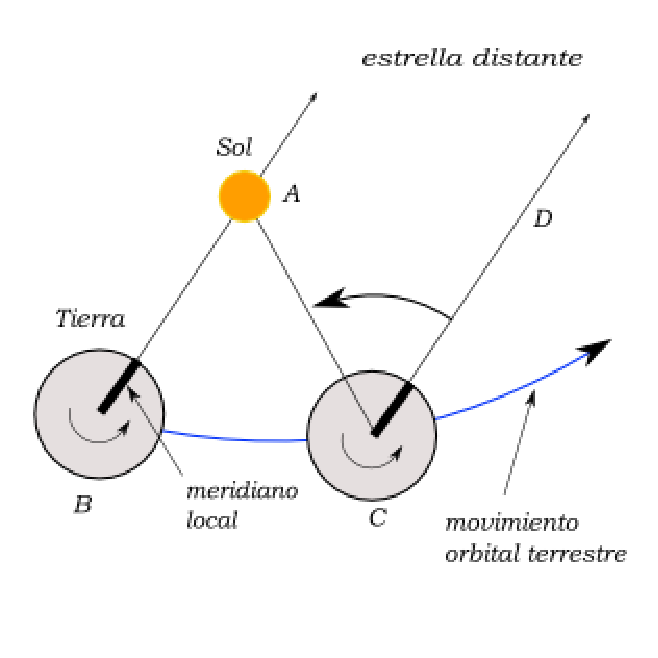
\includegraphics[scale=0.7]{tmp.eps}
 \caption{Situaci\'on estrella-tierra}
 %\label{fig:yeti}
\end{figure} 

Por lo que existen sistemas de coordenadas especiales como son Sistema de coordenadas 
Horizontales, Ecuatoriales, Ecl\'ipticas, entre otras, para poder simplificar 
esta situaci\'on. Estos sistemas de coordenadas usan como referencia la hora actual, 
ubicaci\'on geogr\'afica y otros factores para realizar las conversiones entre ellas.
 Adem\'as de estas condiciones existe una gran cantidad de cosas que afectan el poder
realizar este tipos de observaciones, como son la luz solar, que da\~na los telescopios, 
algunas condiciones clim\'aticas, la luminosidad de la luna, entre otras cosas, lo que 
hace que los operadores de telescopios est\'en sumamente atentos a estos importantes 
acontecimientos que pueden da\~nar gravemente el telescopio. Actualmente existen
c\'upulas para los telescopios que tienen la funci\'on de proteger el telescopio y 
la instrumentaci\'on cient\'ifica, al tiempo que sigue sus movimientos y le permite 
explorar la b\'oveda celeste.
\newpage
\begin{figure}[h!]
 \centering
 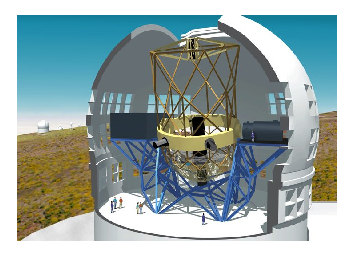
\includegraphics[scale=1.5]{cup.eps}
 \caption{C\'upula que protege el telescopio}
 %\label{fig:yeti}
\end{figure}

Despu\'es de esta peque\~na descripci\'on podemos apreciar que para poder manejar 
un telescopio se necesitan d\'ias de preparaci\'on antes de poder trabajar con 
\'el, ya que sus interfaces son complicadas y muy detalladas y para cada telescopio 
existe una interfaz distinta, implementada de diferente forma, dependiendo del lugar
en donde se cre\'o, por esto mismo, puede estar en diversos idiomas. Un ejemplo de 
una interfaz es la que se muestra en la figura 3.

\begin{figure}[h!]
 \centering
 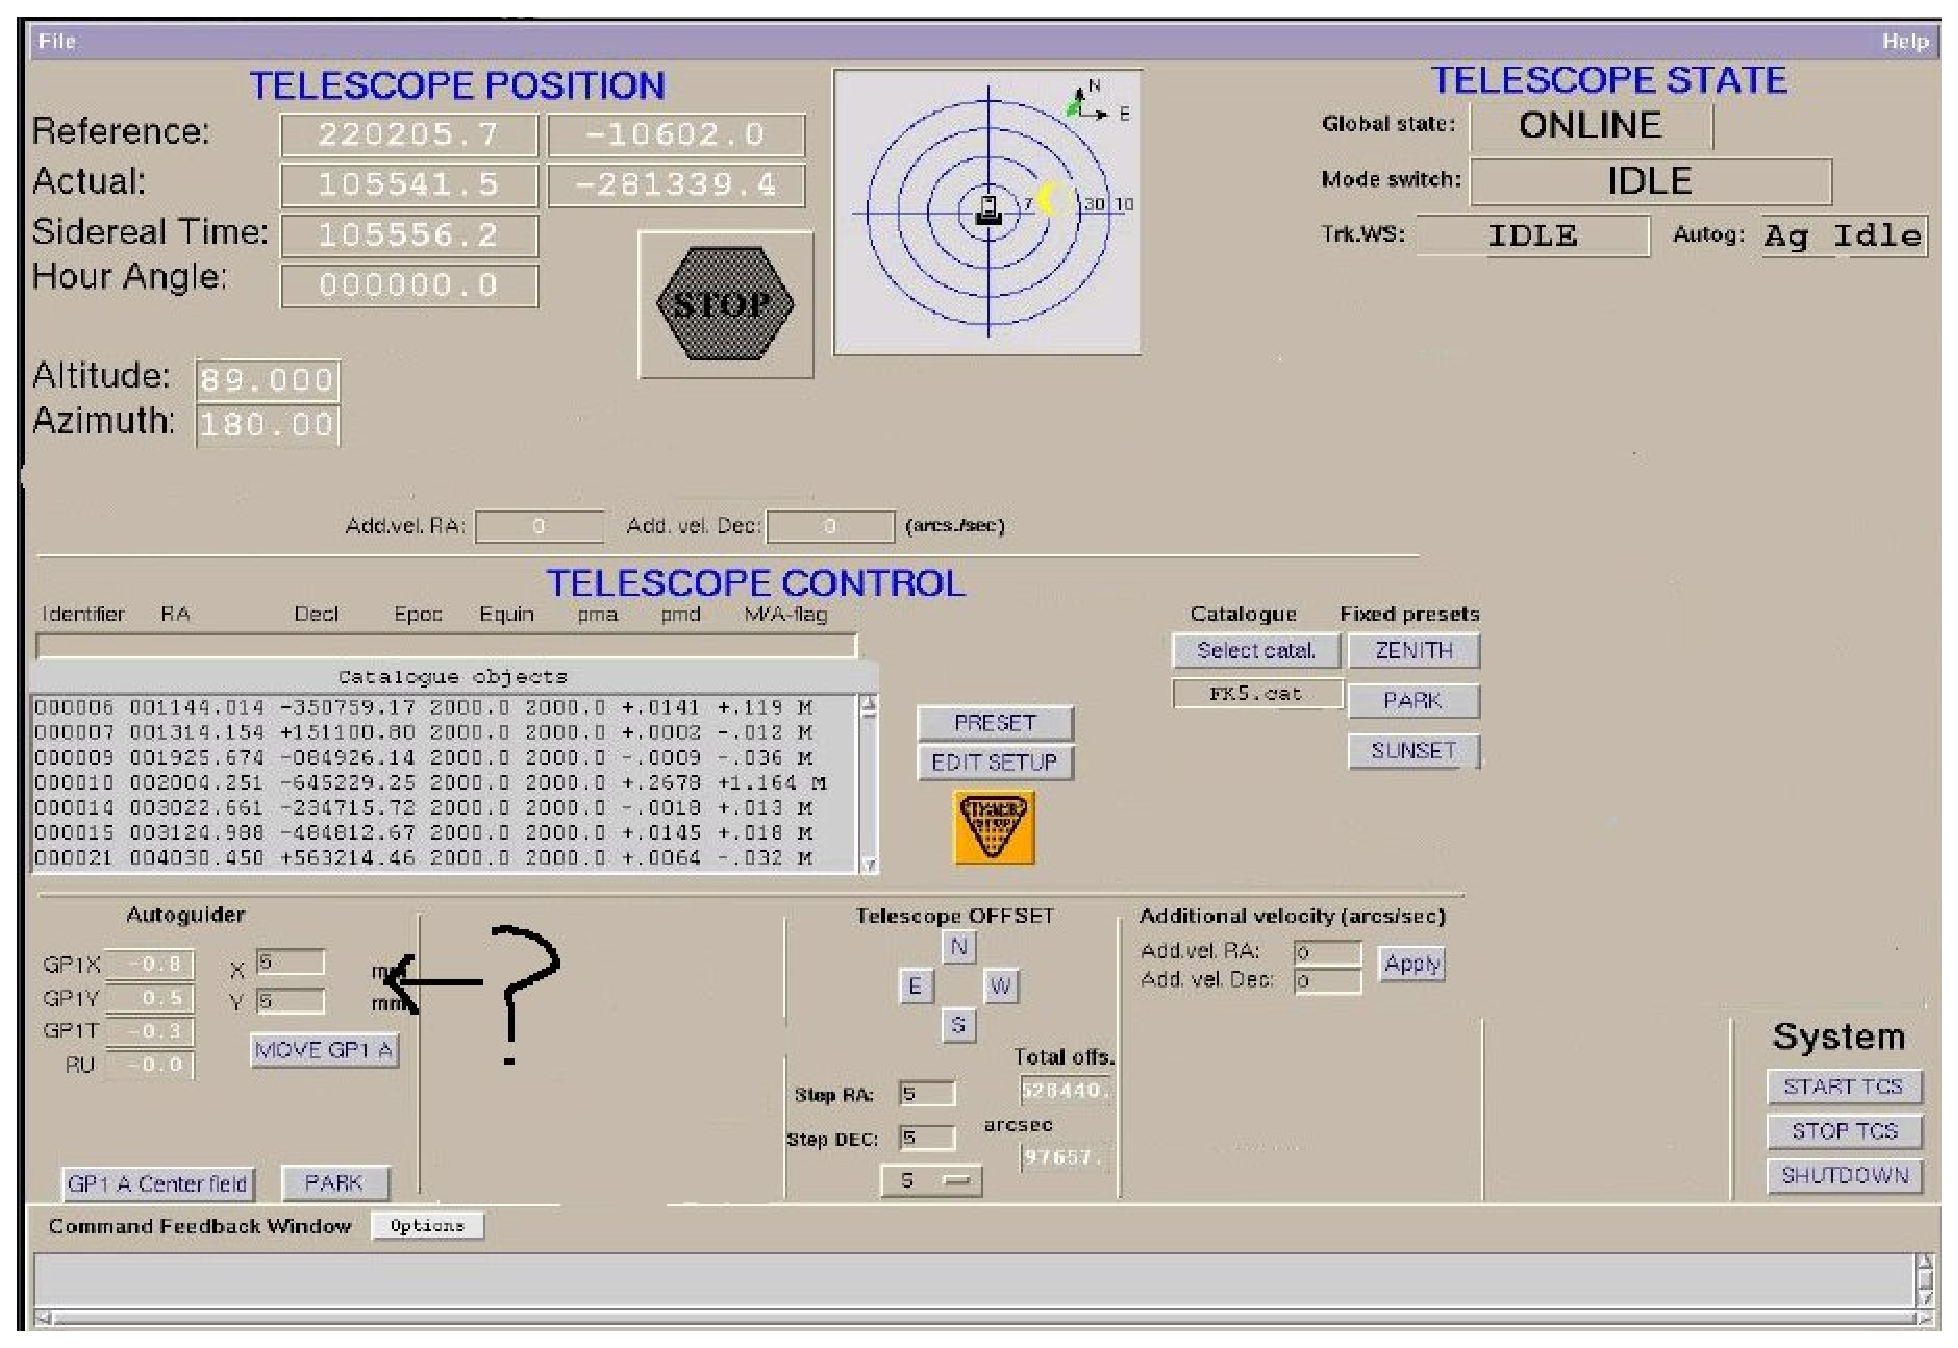
\includegraphics[scale=0.5]{tele.eps}
 \caption{Interfaz de un telescopio}
 %\label{fig:yeti}
\end{figure}

Podemos observar la confusi\'on que puede lograr y lo poco amigable que son estas 
interfaces actualmente y, en en la mayoria de los casos, tienen la informaci\'on 
necesaria para un operador de telescopio pero de forma desordenada y poco est\'andar.
 Como la mayor\'ia del tiempo el astr\'onomo est\'a en busca de nuevos descubrimientos 
que ayuden al entendimiento del universo, no se centran mucho en observar estrellas 
ya existentes, m\'as que para referencias para observar algo que podr\'ia estar 
cerca de ellas y, para ello, deben consultar cat\'alogos de estrellas, siendo un 
retraso la b\'usqueda de ella en el tiempo de observaci\'on.

\subsubsection{Identificaci\'on de problemas y deficiencias}
\textbf{Unicidad de Software:} En la actualidad existen diversos tipos de telescopios, 
los cuales est\'an implementados de manera diferente dependiendo de su dise\~nador o 
de d\'onde fueron creados. Junto con esto, aparece el problema de que cada telescopio 
posee una aplicaci\'on diferente para su control, lo que obliga a los astr\'onomos, 
operadores de telescopios y aficionados a utilizar gran parte de su tiempo aprendiendo 
a ocupar los distintos softwares para cada uno de los equipos con los que van a trabajar.

\textbf{Control:} Actualmente el control de los telescopios se debe hacer de forma local, 
es decir, los operadores de telescopios y astr\'onomos deben estar en el observatorio 
para realizar sus investigaciones, pudiendo hacerse \'este de forma remota, mejorando 
la situaci\'on para los astr\'onomos, especialmente para los que se encuentran lejos 
de los sitios de observaci\'on.

\textbf{Dificultad de Uso:} Muchos de los programas utilizados actualmente para control 
de telescopios son bastante complicados de usar, obligando a gastar una considerable 
cantidad de tiempo aprendiendo a usarlos y, tambi\'en, a usarlos frecuentemente para no 
olvidar c\'omo es que se hace.

\textbf{Seguridad del telescopio:} Es importante que el telescopio tenga medios para 
protegerse de los distintos eventos que puedan ocurrir: luminosidad alta, clima inadecuado, 
entre otros. 

\newpage

\subsection{Caracterizaci\'on del cambio}
\subsubsection{Caracter\'icticas y Potencialidades deseadas}


\paragraph{Caracter\'isticas espec\'ificas deseadas para el producto.}

	\begin{itemize}
	\item \textbf{Control por internet de telescopios:} Se quiere que el sistema 
pueda funcionar situado en cualquier parte del mundo permitiendo controlar alg\'un 
telescopio que se encuentre en otro lugar geogr\'afico.

	\item \textbf{Interfaz Gr\'afica:} El software de control de telescopios debe 
tener una interfaz agradable a los usuarios y permitir el acceso eficiente a las 
funcionalidades que se requieran, adem\'as, debe mostrar siempre en pantalla la 
informaci\'on de mayor importancia.

	\item \textbf{Reproducci\'on de lo que ve la c\'amara:} El sistema debe 
mostrar a donde apunta el telescopio en todo momento de observaci\'on, por medio de 
la c\'amara CCD.

	\item \textbf{Interacci\'on con ACS:} Es necesario que el sistema interact\'ue con 
los telescopios por medio de ACS, de manera que \'este sea el que se conecte 
directamente con los observatorios y telescopios.

	\item \textbf{Ajustar posici\'on del telescopio bajo sistema de coordenadas 
ecuatoriales:} El sistema debe poder recibir las coordenadas que se quiere observar 
y convertirlas a las coordenadas que utiliza el telescopio para poder moverlo a esa 
direcci\'on.

	\item \textbf{Mover el telescopio a la hora sideral:} El sistema debe tener la 
funcionalidad de seguir la posici\'on que se est\'a observando, ya que si no se 
hace, parecer\'ia que lo observado se ve desplazando.

	\item \textbf{Impedir observaciones a lugares con luminosidad lunar:} El sistema 
debe evitar que el telescopio apunte a direcciones con notoria luminosidad lunar, 
debido a que esta luminosidad puede da\~nar severamente los lentes del telescopio.

	\item \textbf{Mostrar modelo visual del telescopio:} Debido a que el telescopio se 
quiere manipular de forma remota, es necesario otorgar alguna forma que permita 
ver a la persona que lo est\'e operando, en qu\'e estado se encuentra. Para esto, 
el sistema debe tener un modelo visual que se comporte de la misma forma que lo 
hace el telescopio real.

	\item \textbf{Ajuste manual del telescopio:} El sistema debe permitir controlar el 
telescopio manualmente para permitir ajustes menores, que ayuden a corregir errores 
en la direcci\'on que se observa, que pudieran ocurrir por factores externos, como 
es la deflexi\'on por el peso propio del telescopio en algunas posiciones.

	\item \textbf{Detener de forma inmediata el telescopio en caso de emergencia:} El 
sistema tiene que tener una opci\'on de emergencia para detener el telescopio de 
forma inmediata para evitar cualquier da\~no que se crea que pueda ocurrir. Por 
ejemplo, da\~no por alguna variaci\'on en las condiciones clim\'aticas.

	\item \textbf{Controlar acceso a la aplicaci\'on (Sesiones):} El sistema debe tener 
acceso para los distintos usuarios, de manera que cada uno tenga su propia 
estad\'istica de lo observado.

	\item \textbf{Guardar coordenadas de observaci\'on realizadas:} El sistema debe 
guardar registro de las coordenadas observadas por cada usuario del sistema. De 
esta forma ayuda a que se puedan repetir observaciones y a realizar estudios sobre 
\'estas.

	\end{itemize}


\newpage

\paragraph{Relaci\'on de las caracter\'isticas con los problemas identificados.}

	\begin{itemize}

	\item El control por internet va a ayudar a solucionar el problema de tener 
que estar en el lugar de observaci\'on al momento de controlar al telescopio.

	\item La interfaz gr\'afica va a ayudar a disminuir la dificultad de uso, 
ocultando informaci\'on que no sea requerida en todo momento, pero permitiendo 
verla de manera sencilla e intuitiva.

	\item La reproducci\'on de lo que est\'a viendo el telescopio es de gran 
utilidad para la experiencia remota, debido a que sino hiciera esto, no se podr\'ia 
ver lo que est\'a viendo el telescopio, hasta que se enviara alg\'un informe a 
quien controlaba el telescopio.

	\item La interacci\'on con ACS es una de las caracter\'isticas principales 
para el control gen\'erico de telescopios y el control de telescopios por medio 
de internet, pues es esta plataforma la que permite la comunicaci\'on con los 
telescopios en los diferentes observatorios del mundo.

	\item Mover el telescopio a la hora sideral reduce la dificultad de uso 
para el seguimiento de la observaci\'on de alg\'un objeto, puesto que nos permite 
ver en todo momento al objeto deseado, sin necesidad de realizar tareas adicionales.

	\item Al impedir que el telescopio apunte a lugares con luminosidad lunar 
se reduce la dificultad de uso, puesto que no es necesario estar preguntandose 
todo el tiempo si el telescopio va a apuntar a lugares potencialmente da\~ninos 
para el mismo. Adem\'as, aumenta la seguridad del telescopio puesto que lo proteje 
de la luz lunar, uno de los factores m\'as comunes que da\~nan al telescopio.

	\item El modelo visual soluciona un aspecto muy importante de la facilidad 
de uso para el control a trav\'es de internet, ya que con este se puede saber en 
todo momento hacia d\'onde est\'a apuntando f\'isicamente el telescopio, d\'andonos 
un apoyo gr\'afico de lo que estamos haciendo. De la misma forma, tambi\'en ayuda 
a los que operan el telescopio de forma local, aunqiue ellos podr\'ian verlo 
directamente, puede ser m\'as c\'omodo verlo en la misma pantalla que est\'an trabajando.

	\item El ajuste manual ayuda a disminuir la dificultad de uso del sistema, 
puesto que con este, no es necesario intuir una direcci\'on parecida a la que 
estamos observando de manera que se vea lo que debiera, sino que simplemente 
lo movemos manualmente hasta donde debiera estar.

	\item Al dar la posibilidad de detener manualmente al telescopio, aumentamos 
en gran medida su seguridad, puesto que mediante esta opci\'on, podemos protegerlo 
de factores que no esperabamos, como son las variaciones inesperadas en el clima. 

	\item El guardar coordenadas de observaci\'on realizadas por sesi\'on facilita 
la dificultad de uso del sistema, ya que para gente no muy experimentada en el tema, 
permite repetir las observaciones hechas otros d\'ias.

	\end{itemize}


\subsection{An\'alisis de las alternativas de soluci\'on}
\subsubsection{Alternativa 1: Desarrollo de Software basado en ACS} %%%% TOMAS
Desarrollo de un producto de software basado en la plataforma ACS que sea gen\'erico,
es decir, que nos permita controlar cualquier telescopio por medio del mismo
programa, sin la necesidad de tener un programa diferente para cada telescopio.

Se utiliza un computador como estaci\'on de trabajo de quien opere el telescopio, 
en donde todo el control se realizar\'a por medio de una interfaz gr\'afica. Este
computador requerir\'a tener acceso a internet para poder obtener componentes desde
ACS y para comunicarse con el telescopio que se quiera controlar.

La interfaz gr\'afica mostrar\'a a quien opere el telescopio el estado actual del
mismo, pudiendo verse lo que est\'a observando el telescopio por medio de la
c\'amara CCD y la disposici\'on f\'isica en que se encuentra el telescopio, por medio
del modelo hecho en OpenGL del mismo.

Es importante notar que al utilizar la plataforma ACS para la distribuci\'on de 
componentes de software, se podr\'ian usar componentes realizados por otras personas, 
asi como realizar cambios en componentes que utiliza nuestro software, obteniendo un
producto de alta modularidad, enfocado al trabajo por componentes.

\subsubsection{Alternativa 2: Reutilizaci\'on de software de control de telescopios} %%%% TODOS
Realizar un programa que reutilice las aplicaciones existentes detectando el telescopio
que se quiere controlar y luego llamando a la aplicaci\'on correspondiente.

En m\'as detalle, consiste en realizar una base de datos que contedr\'ia una 
asociaci\'on entre los telescopios y el programa que los controla. Para reducir
el tama\~no de las distribuciones se utilizar\'ia un sistema distribuido de los
distintos programas, de manera que cuando se detecte el telescopio que se quiera
controlar, se haga una petici\'on de descarga el software requerido para su control.

En esta soluci\'on aparecen muchos problemas, destacando los problemas legales en 
cuanto a tema de patentes y derechos de autor, los problemas de diferencia de 
interfaz gr\'afica, recursos necesarios del equipo poco claros y variables seg\'un 
el telescopio que se controle.

De los derechos legales lo principal ser\'ia el tema de las patentes y los derechos
de autor, ya que utilizar\'iamos programas hechos por otras personas que muchas 
veces tienen patentes y est\'a restringido su uso por decisi\'on de sus autores. 
Por la gran cantidad de programas existentes, nos ser\'ia imposible hacer peticiones 
a cada uno para usar su programa.

Debido a que en esta soluci\'on llamamos a programas hechos por otras personas, para
cada telescopio tendr\'iamos una interfaz gr\'afica diferente, lo cual deja uno de 
los principales problemas sin mejorar.

Ya que se utilizan distintos programas dependiendo del telescopio que se quiera 
controlar, no podr\'ia asegurarse los requerimientos del equipo para el control del
telescopio. Se podr\'ia poner el mayor de los casos, pero no es lo m\'as adecuado.

\subsection{Soluci\'on recomendada} %%%% TOMAS
La mejor soluci\'on que encontramos es la alternativa 1, en la cual se piensa construir
un producto de software gen\'erico basado en ACS, el cual se acopla bastante bien 
con las características requeridas.

Este producto deber\'a ser modular basado en componentes con el estilo que ACS nos
impone, por lo que se tendr\'an algunos componentes sobre esta plataforma, mientras que
otros ir\'an junto con el software principal. Es importante hacer la separaci\'on
de las capas de comunicaci\'on, interfaz gr\'afica y software, para simplificar la
mantenci\'on del producto al tener las funcionalidades separadas.

Se eligi\'o esta alternativa, porque en la actualidad no hay productos que controlen
telescopios de forma gen\'erica, y esto es algo muy importante para enfocar los esfuerzos
de observaci\'on en las observaciones mismas y no en aprender a utilizar los programas
asociados al control de telescopios.


\newpage
\section{T\'ecnicas y Herramientas de desarrollo} %%% CARLOS
\subsection{Modelo de desarrollo}
Las caracter\'isticas m\'as importantes del proyecto Hevelius con
respecto a la elecci\'on de un modelo de desarrollo se expone en lo
siguiente. Primero se consideran las propiedades del producto:

\begin{itemize}
\item \textbf{Complejidad del Proyecto:} una estimaci\'on informal del proyecto
  muestra una complejidad media, la cual permite la finalizaci\'on del
  proyecto dentro del plazo predeterminado;
\item \textbf{Solidez de los Requerimientos:} c\'omo el producto a
  desarrollar est\'a inserto en un proyecto de investigaci\'on, es posible que
  los requerimientos capturados durante el an\'alisis sean completos en su generalidad,
  sujetos a pocos cambios.
\item \textbf{Innovaci\'on del Producto:} en vista de que la principal caracter\'istica
  del proyecto es la b\'usqueda de la generalidad en el control de telescopios, existen 
  errores que durante el desarrollo se descubrir\'an, lo que nesecitar\'a cambios en el
  c\'odigo implementados o en el dise\~no del software.
\end{itemize}

Adem\'as, el ambiente del desarrollo tiene las siguientes caracter\'isticas:

\begin{itemize}
\item \textbf{Tama\~no del Equipo:} cuatro personas durante la planificaci\'on y el 
  desarrollo del proyecto.
\item \textbf{Tratamiento de los miembros del equipo entre s\'i:} informal, ya
  que existen lazos de amistad anteriores a la formaci\'on del grupo de trabajo.
\item \textbf{Proyecci\'on en el tiempo:} se cuenta con un plazo determinado,
  debido a que el proyecto pretende ser parte de la Feria de Software 2007, 
  de aproximadamente cinco meses a partir de la fecha de entrega de este informe.
\end{itemize}


Teniendo en cuenta el conjunto de caracter\'isticas del proyecto, se
decide usar un modelo de desarrollo en fases para la
mayor\'ia de las tareas; espec\'ificamente se prevee el uso del \emph{Modelo
Iterativo} en el trabajo. Sin embargo, no podemos desechar el \emph{Modelo
Incremental}, debido a la posible implementaci\'on de m\'odulos no considerados en un
principio en el software.

Habiendo elegido este m\'etodo de desarrollo, es necesario realizar las
siguientes actividades durante el desarrollo para el modelo iterativo:

\begin{enumerate}
\item \textbf{Pruebas:} los requerimientos (funcionales o no-funcionales) deben
  ser transformados en pruebas automatizables.
\item \textbf{Construir:} el c\'odigo producido debe estar siempre en un
  estado que permite su compilaci\'on.
\item \textbf{Dise\~nar:} para facilitar el proceso de codificaci\'on y permitir el
  trabajo paralelo de grupos independientes, hay que contar con un
  dise\~no del sistema.
  Esta actividad hay que hacerla durante todo el tiempo del desarrollo,
  adapt\'andose a funcionalidad agregada.
\item \textbf{Comunicaci\'on dentro del equipo:} es importante
  que la comunicaci\'on entre los integrantes funcione
  muy bien, es decir, todos deben saber la mayor\'ia del tiempo en qu\'e
  est\'an trabajando los dem\'as y cu\'ales son los cambios realizados por
  ellos.
\end{enumerate}

Para el componente planificado, hay que hacer un plan inicial de
recursos y tiempo necesitado, para lo que sirve este documento, y
controlar el progreso actual del proyecto, para lo que sirven los
\emph{fichas de estado}.

Adem\'as es necesario documentar el dise\~no actual del programa.


\subsection{Herramientas y t\'ecnicas de soporte para el desarrollo}
\subsubsection{T\'ecnicas a utilizar en el desarrollo del proyecto}

Durante el desarrollo del proyecto se utilizar\'a el m\'etodo de desarrollo en fases iterativo, 
ya que como hay ejecutables desde el mismo comienzo del proyecto, pueden ser examinados 
para proponer cambios si fuera necesario. Tambi\'en la empresa tiene una r\'apida 
retroalimentaci\'on de lo que funciona y lo que no, ya que las pruebas se realizan desde el 
comienzo mismo del proyecto y no se debe esperar al final para hacer las modificaciones necesarias.\\

Se opt\'o por este m\'etodo debido a la seguridad que da su planificaci\'on, ya que se 
puede \textit{ver} en que se est\'a trabajando y cuales ser\'an los pr\'oximos pasos a seguir.\\

Se requiri\'o el uso de ciertos lenguajes 
de programaci\'on, debido a est\'andares internacionales. Estos lenguajes son: C, C++, Java y Phyton. 
Todos los integrantes del grupo, cuentan con conocimientos en C, Java y otros en C++.\\

Es posible que se utilice alguna herramienta de dise\~no vectorial para la creaci\'on de las gr\'aficas 
a utilizar en el software, pero a\'un no se ha descartado ni confirmado ninguna de ellas.\\


\subsubsection{Herramientas o plataformas espec\'ificas a utilizar}

La plataforma operacional de Hevelius est\'a constituida por el Sistema Operativo Linux Fedora Core, 
debido a que es esta la distribuci\'on utilizada para desarrollar software. Esta 
distribuci\'on a su vez debe contar con el framework ACS en su versi\'on 6.0 o superior.\\



\newpage
\section{Implementaci\'on (Entrega y Operaci\'on)} %%% MARINA
\subsection{Plan de operaci\'on del sistema}
Los componentes computacionales m\'inimos requeridos por Hevelius para su 
operaci\'on consisten en un computador con Sistema Operativo Linux Fedora Core 
y Software ACS 6.0, no se restringe s\'olo a la utilizaci\'on de esta versi\'on, puede 
utilizar otras, pero con las distintas versiones puede ser que existan variaciones 
que impliquen modificaciones al c\'odigo fuente, pero se deja 
establecido que en la versi\'on 6.0 funcionar\'a correctamente, de acuerdo 
a los requerimientos.

El equipo en el cual se implemente Hevelius tambi\'en debe poseer acceso 
a Internet y sin olvidar el acceso al telescopio que se desea operar. Sobre 
los requerimientos m\'inimos de hardware a\'un no est\'an definidos.

Hevelius se desarrollar\'a sobre la plataforma Linux Fedora Core y Software ACS 6.0 como 
ya se hab\'ia especificado y con el telescopio NEXSTAR 4 SE y a\~nadido 
a \'este una c\'amara CCD para la obtenci\'on de im\'agenes.

Como Hevelius es s\'olo el primer paso para el desarrollo completo de un 
software de control gen\'erico para telescopios, es muy importante la 
comprensi\'on del c\'odigo entregado, debidamente comentado y, como requerimiento 
adicional, en ingl\'es.

\subsection{Plan de implementaci\'on (entrega)}
Una vez finalizado el desarrollo del software, el proceso de entrega debe 
consistir de dos fases.

\begin{enumerate}
	\item {\bf{Entrega del programa y c\'odigo.}}\\
Como ya se ha mencionado anteriormente Hevelius es un paso a la construcci\'on 
de un software gen\'erico, es por ello la importancia del c\'odigo, puesto que 
es la base para que posteriormente se siga desarrollando en este tema, por 
estas razones se entrega el c\'odigo debidamente ordenado, organizado y 
comentado en ingl\'es.

En lo que se refiere al programa en s\'i, no se puede hacer una capacitaci\'on 
a quienes usar\'an este software, ya que no son personas espec\'ificas. Pero al 
finalizar el desarrollo de Hevelius se tratar\'a que astr\'onomos prueben el 
funcionamiento del software. Es por esto, que para aquellos que deban tratar 
con Hevelius, existe una documentaci\'on en la cual se detalla los componentes 
y la utilizaci\'on de ellos, esta documentaci\'on ser\'a especificada en la 
siguiente fase.\\

	\item{\bf{Documentaci\'on.}}\\
Como Hevelius est\'a siendo creado para personas especializadas en el tema de 
la astronom\'ia, se les entrega documentaci\'on detallada del software, ya que 
no existe una instancia directa en donde se pueda preguntar acerca de su 
funcionamiento, donde el \'unico contacto podr\'ia ser mediante correo 
electr\'onico, puesto que el ambiente en que trabaja Hevelius es el de los 
observatorios y, por lo tanto, el trato directo se hace m\'as complicado.

La especificaci\'on de la documentaci\'on consiste en las siguientes partes:

\begin{itemize}
	\item {\bf{Explicaci\'on de la interfaz:}} Esta consiste en la 
explicaci\'on de d\'onde se encuentra ubicado cada uno de los componentes que 
tiene implementado Hevelius.
	\item{ \bf{Componentes Implementados:}} En una secci\'on se especifica 
qu\'e hace cada uno de sus componentes y c\'omo es el funcionamiento de ellos, 
qu\'e par\'ametros recibe, etc.

Toda la documentaci\'on debe ser desarrollada en ingl\'es.
\end{itemize}
\end{enumerate}

\subsection{Plan de mantenci\'on}
Como ya se ha mencionado anteriormente Hevelius esta implementado mayormente 
para observatorios, los cuales se encuentran en distintas partes del mundo y 
los usuarios del programa pueden acceder desde donde prefieran para manipular 
los telescopios, por lo que nos es imposible dar mantenimiento presencial a 
todos los usuarios.\\

Puede existir una asistencia remota, principalmente a trav\'es de correo 
electr\'onico para tratar de resolver cualquier tipo de problema que pueda 
existir.
A dem\'as contamos con la asistencia de ACS-UTFSM Group, quienes se encargar\'ian 
de la manteci\'on de Hevelius, as\'i como el soporte en caso de detectarce 
BUGS dentro del software.

\end{document}
